% !TeX spellcheck = da_DK
\chapter{Android udvikling}

Når vi snakker om Android, så snakker vi om et "styresystem". Det kan man anskue som et kæmpe stort program, der administrerer alle de apps der kører på mobilen. I denne bog, bruger vi begreberne "styresystem" og "platform" i flæng.

De eneste relevante styresystemer til mobiler er pt. følgende to:

\begin{itemize}
	\item IOS (IPhone, IPads etc.)
	\item Android (Samsung, HTC, Sony etc.)
\end{itemize}

På SDC, kigger vi på den sidste af de to, nemlig Android udvikling. Selvom app-udvikling til IOS og Android minder meget om hinanden, så er der en række væsentlige forskelle i de værktøjer man bruger. Derfor kigger vi kun på den ene af de to styresystemer.

\section{Hvad er Android apps?}
Når man skal beskrive hvad en "Android app" er, så kan det gøres lidt simplere ved at forstå hvad en "app" er. App er en forkortelse for applikation, hvilket på godt gammeldags jydsk er synonymt med "et program". Når vi snakker om en app, snakker vi derfor om et computer program, som er kodet med en række instruktioner.

I Android verdenen, er stort set alt apps. Lige fra låseskærmen og "indstillinger" menuen til Super Mario Go, og Farmville. Derfor er der meget få grænser for hvad man kan opnå ved app-udvikling til Android.

\marginfigure{xkcd_app.png}{Billede lånt af: \url{https://xkcd.com}}

\subsection{Anatomien af en Android app}
Android apps består af mange forskellige dele. De primære dele kan dog deles op i følgende tre kategorier:

\subsubsection{Ressourcer}
Ressourcer er indstillinger, billeder, layouts (se \autoref{sec:android:layouts}) og alt mulig andet data der bruges i en app. De findes i mappen \texttt{res/} og har forskellige undermapper, afhængig af hvilken type ressource det er.

\subsubsection{Activities}
Activities er aktiviteter man kan foretage sig i app'en. Der kan f.eks. være en "tag billede" activity, en "gem billedet" activity og en "se dit galleri af billeder" activity. Disse activities vil blive udforsket yderligere i \autoref{activities kapitel}.


\subsubsection{Manifest}
Et app-manifest er en beskrivelse af app'en som Android styresystemet gør brug af når den kører app'en på mobilen. I manifestet beskriver man hvilke rettigheder app'en har brug for, samt hvilke teknologier den gør brug af.

Derudover kan manifestet indeholde information om hvordan andre apps kan kommunikere med denne app, og andre indstillinger der binder app'en sammen med resten af platformen.

\section{Layouts}
\label{sec:android:layouts}

Layouts er en ressource som app'en gør brug af når den skal vise den grænseflade\footnote{En grænseflade er, i denne kontekst, det grafiske design som brugeren interagerer med. Det kan f.eks. være en menu med knapper, eller et billede.} som brugeren skal se på inde i app'en. Det er en beskrivelse af strukturen i app'ens grænseflade.

For bedre at forstå layouts, skal vi først forstå den måde vi skriver et layout på. Ligesom med programmeringssprog, hvor vi har forskellige sprog til at beskrive kode på (som f.eks. Java), findes der forskellige måder at beskrive strukturer og layouts. Vi kalder disse sprog for \textit{strukturelle sprog}, en af de mere udbredte af sådanne sprog er det man kalder for \textit{XML}\footnote{e\textbf{X}tensible \textbf{M}arkup \textbf{L}anguage}.

\subsection{XML}
I sin kerne er XML et meget simpelt sprog. Det er bygget op af "tags". Der er to slags tags, et "opening-tag" og et "closing-tag". Opening-tags er skrevet ved at have et "mindre-end" tegn ($<$), efterfulgt af noget tekst og så afsluttet med et "større-end" tegn ($>$). For eksempel, er følgende et opening-tag: \XmlInline|<Button>|.

Closing-tags er meget lig opening-tags, der er blot en skråstreg efter "mindre-end" tegnet, for at indikere at dette tag lukker et opening-tag der er skrevet tidligere i dokumentet. Et eksempel på et closing-tag, der lukker det opening-tag der var i det tidligere eksempel, kan ses her: \XmlInline|</Button>|.

Det er vigtigt at man altid lukker sine tags. Man må aldrig have et opening-tag uden at det bliver lukket, og man må aldrig have et closing-tag der ikke har noget opening-tag at lukke.

Man kan tilknytte "attributter" til sine opening-tags. Det gør man ved at skrive navnet på attributten, efterfulgt af et lig-med tegn, efterfulgt af attributtens værdi. Denne værdi er typisk skrevet inden i to gåse-øjne ("). Et eksempel på et opening-tag med en attribut er følgende: \XmlInline|<Button Text="Hej med dig!">|.

Et eksempel på et XML dokument ses herunder. Det beskriver et vindue, med en "label" dvs. et kort stykke tekst, med to knapper. Vi har skrevet de tags, der hører til vores label og knapperne, imellem vinduets opening- og closing-tags. Dette betyder at de kommer til at høre til vinduet, altså at vinduet har en label og to knapper. Denne relation bliver ofte beskrevet som at vinduet er forældreren til de tre børn (label og de to knapper).

\begin{example}\noindent
	\begin{XmlCode}{Et lille XML dokument}{first-valid-xml-document}
		<Window>
			<Label Text="Vil du lukke vinduet?"></Label>
			<Button Text="Ja"></Button>
			<Button Text="Nej"></Button>
		</Window>
	\end{XmlCode}
\end{example}


For at simplificere XML dokumentet, kan vi udnytte os af et så-kaldt self-closing tag. Altså et opening-tag der lukkes med det samme, uden man behøver at bruge et closing-tag. Dette skrives ved at putte en skrå-streg ind før "større-end" tegnet:

\begin{example}\noindent
	\begin{XmlCode}{Et lille XML dokument med self-closing tags}{self-closing-tags-dokument}
		<Window>
			<Label Text="Vil du lukke vinduet?"/>
			<Button Text="Ja"/>
			<Button Text="Nej"/>
		</Window>
	\end{XmlCode}
\end{example}

\begin{remark}
	Bemærk at vi ikke kunne bruge et self-closing tag til vores \XmlInline|<Window>| tag, fordi at det ikke skulle lukkes med det samme, da det skulle indeholde dets tre børn.
\end{remark}

Bemærk at vi ikke kunne bruge et self-closing tag til vores \XmlInline|<Window>| tag, fordi at det ikke skulle lukkes med det samme, da det skulle indeholde dets tre børn.

Vi har nu taget en kort intro til XML, det er faktisk et meget mere komplekst sprog end det vi har gennemgået her, men det burde ikke blive nødvendigt at forstå det hele for det vi skal arbejde med her.

Hvis man gerne vil lære mere om XML, kan man besøge W3Schools: \url{https://www.w3schools.com/xml/}.


\subsection{Hvad er layouts?}
Layouts er, som nævnt, en måde at beskrive app'ens udseende på igennem det strukturelle sprog XML.

Vi lægger layouts i ressource mappen \texttt{res/layout/}, og et layout er faktisk bare et XML-tag der kan indeholde andre tags. De beskriver hvordan flere visuelle elementer skal pladseres i forhold til hinanden.

\subsubsection{Frame layouts}

Det første eksempel på et layout er det såkaldte \textit{frame layout}, det er et meget simeplt og effektivt layout der er designet til at pladsere et enkelt element et specifikt sted på skærmen.

Det er svært at håndtere dette layout hvis det har mere end et barn. Derfor bør det typisk kun indeholde et enkelt barn. Deraf kommer navnet "frame", det bruges som en "ramme" til et andet element.

I \autoref{fig:android:layouts:frame-layout} er der et eksempel på hvordan man 
kan have to ``børn'' indeni et frame layout, for at placere det ene oven på det 
andet.

\begin{figure}[h]
	\begin{center}
		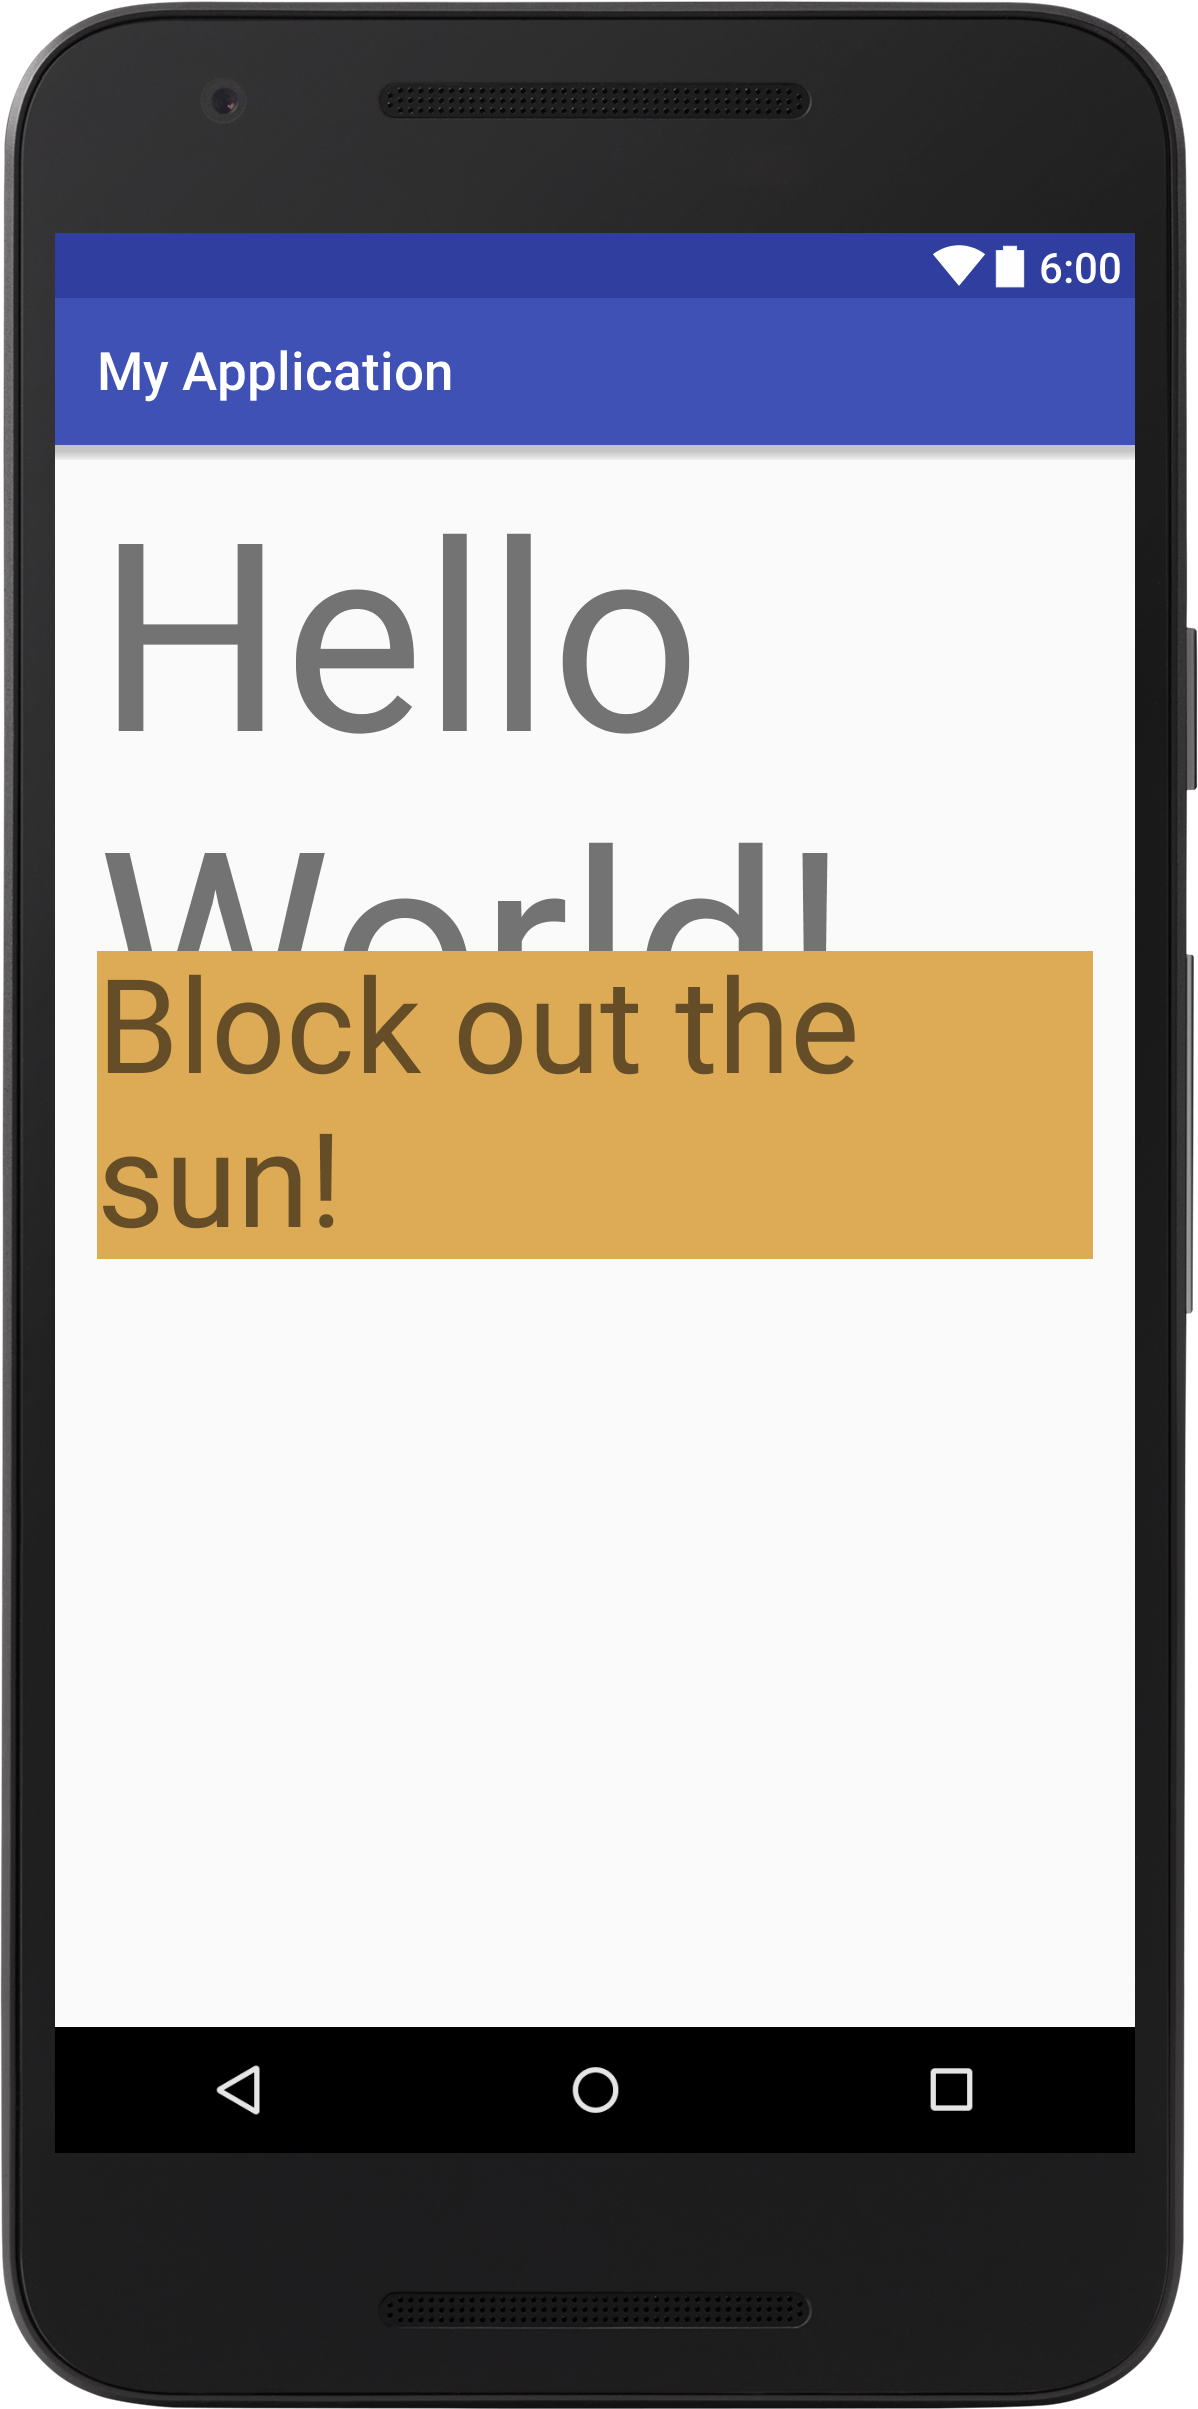
\includegraphics[width=5cm]{frame_layout.png}
		\caption{Et frame layout i en app}
		\label{fig:android:layouts:frame-layout}
	\end{center}
\end{figure}

\begin{XmlCode}{Det layout der giver udseendet i \autoref{fig:android:layouts:frame-layout}}{frame-layout}
	<?xml version="1.0" encoding="utf-8"?>
	<FrameLayout xmlns:android="http://schemas.android.com/apk/res/android"
		xmlns:tools="http://schemas.android.com/tools"
		android:layout_width="match_parent"
		android:layout_height="match_parent"
		android:paddingBottom="@dimen/activity_vertical_margin"
		android:paddingLeft="@dimen/activity_horizontal_margin"
		android:paddingRight="@dimen/activity_horizontal_margin"
		android:paddingTop="@dimen/activity_vertical_margin"
		tools:context="com.example.lukas.myapplication.MainActivity">
	
		<TextView
			android:layout_width="wrap_content"
			android:layout_height="wrap_content"
			android:text="Hello World!"
			android:textSize="100sp"/>
		<TextView
			android:layout_width="fill_parent"
			android:layout_height="wrap_content"
			android:layout_gravity="center_vertical"
			android:layout_marginBottom="50dp"
			android:background="#ddaa55"
			android:text="Block out the sun!"
			android:textSize="50sp"/>
	</FrameLayout>
\end{XmlCode}

\subsubsection{Linear layouts}

\subsubsection{Tabular layouts}

\begin{exercise}
	Lav et tabular-lignende layout ved hjælp af linear layouts.
\end{exercise}

\begin{exercise}
	Lav et linear-lignende layout ved hjælp af tabular layouts (både horisontalt og vertikalt).
\end{exercise}

\subsubsection{Relative layouts}